The mathematical laws describing the deformation of a solid body are summarized in this section. First, the kinematic laws governing the motion of each material point belonging to a solid are considered. Then \textit{strain} measures are associated to internal forces through the thermodynamic framework so that \textit{constitutive equations} are derived. For a more exhaustive review of governing equations, see for instance \cite{Foundation_of_elasticity}, \cite{Truesdell}, \cite{Simo}, \cite{Belytschko}.

\subsection{Kinematic laws -- Strain measures}
Consider a three-dimensional solid with volume denoted by $\Omega \subset \Rbb^3$ bounded by the surface $\partial \Omega$. This body undergoes external forces that can either be localized on a part of the external surface of the body (\textit{i.e. surface forces}) or act in the whole solid domain (\textit{i.e. volume forces}). Due to the presence of such loads, the domain may change within the time interval $\tau = \[0,T\]$ and is hence written as a function of time $\Omega(t)$ ($t\in \tau$). The state of the solid at time $t=0$, corresponding to a non-deformed state with volume $\Omega(t=0)=\Omega_0$, is referred to as the \textit{initial configuration}. Some problems require the use of a \textit{reference configuration} that can be deformed and to which equations are referred. In what follows, the reference and initial configurations are identical. At a given time $t>0$, the volume is $\Omega(t)=\Omega_t$ and the state of the solid corresponds to the \textit{current configuration}. These configurations are depicted in figure \ref{fig:deformationFunction}.
\begin{figure}[h]
  \centering
  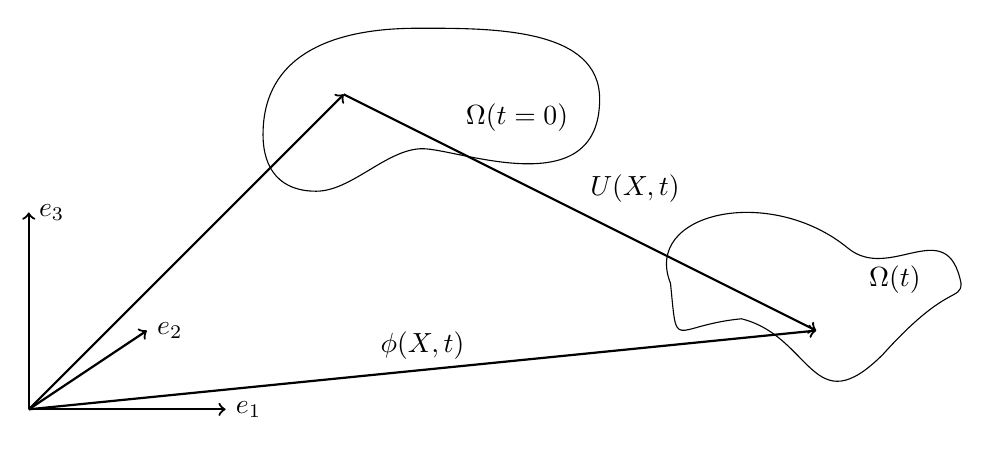
\begin{tikzpicture}
  %\draw[step=1.0,black,thin] (-3.,-1.) grid (3,4.);
  %\draw (-3,-1) -- (3,-1) -- (3,4) -- (-3,4) -- (-3,-1);
  \draw[thick,->] (-5,-2.5) -- (-2.5,-2.5) node [right] {$\vect{e}_1$};
  \draw[thick,->] (-5,-2.5) -- (-5,0.) node [right] {$\vect{e}_3$};
  \draw[thick,->] (-5,-2.5) -- (-3.5,-1.5) node [right] {$\vect{e}_2$};
  \begin{scope}[scale=0.45]
    \draw (-3,0.6) .. controls +(1,0) and +(-1,0) .. (0,1.8)  
    .. controls +(1,0) and +(0,-3) .. (5,3.2) 
    .. controls +(0,2) and +(2,0)  .. (0,5.2) 
    .. controls +(-1,0) and +(0,3) .. (-4.5,2.2) 
    .. controls +(0,-1) and +(-1,0).. (-3,0.6) ;
  \end{scope}
  \node at (1.2,1.2) {$\Omega(t=0)$};
  %% Deformed body +2.
  \begin{scope}[scale=0.9]
    \draw (0.+0.5+4.,0-1.5) ..controls (1.+0.5+4.,-0.25-1.5) and (1.+0.5+4.,-1.5-1.5) .. (2.+0.5+4.,-0.5-1.5) ..controls (2.9+0.5+4.,0.5-1.5) and (3.1+0.5+4.,0.25-1.5) .. (3.1+0.5+4.,0.5-1.5) ..controls (2.9+0.5+4.,1.5-1.5) and (2.1+0.5+4.,.5-1.5) .. (1.5+0.5+4.,1.-1.5) ..controls (0.4+0.5+4.,1.9-1.5) and (-1.4+0.5+4.,1.5-1.5) .. (-1.+0.5+4.,0.5-1.5)..controls (-0.4+0.+4.,-0.-2.) and (-1+0.5+4.,0.4-2.) .. (0+0.5+4.,0-1.5);
  \end{scope}
  \node at (6.,-0.85) {$\Omega(t)$};
  \draw[->,thick] (-5,-2.5) -- (-1.,1.5) node [midway,left] {$\X$};
  \draw[->,thick] (-5,-2.5) -- (5.,-1.5) node [midway,above] {$\vect{\phi}(\vect{X},t)$};
  \draw[->,thick] (-1.,1.5) -- (5.,-1.5) node [midway,above right] {$\vect{U}(\vect{X},t)$};
\end{tikzpicture}

%%% Local Variables:
%%% mode: latex
%%% TeX-master: "../../mainManuscript"
%%% End:
  \caption{Deformation of a solid body between a reference state $\Omega_0$ to a subsequent state $\Omega_t$.}
  \label{fig:deformationFunction}
\end{figure}
The points of $\Rbb^3$ are located with \textit{Eulerian} or \textit{spatial coordinates} $\vect{x}=x_i\vect{e}_i$ while material particles in the reference configuration are located with \textit{Lagrangian coordinates} $\vect{X}=X_\alpha \vect{E}_\alpha$.
%Two different bases $(\vect{E}_1,\vect{E}_2,\vect{E}_3)$ and $(\vect{e}_1,\vect{e}_2,\vect{e}_3)$, that may be different are not, allow the use of \textit{Lagrangian coordinates} and $\vect{E}_\alpha$ or \textit{Eulerian coordinates} $\vect{x}=x_i\vect{e}_i$ respectively. %Lagrangian coordinates give the location of material particles in the reference configuration while Eulerian coordinates are used to locate the point of space at which a particle may be at a given time.
%In the reference configuration, all material particles are located by their position vectors: $\vect{X}=X_\alpha \vect{E}_\alpha$.
At time $t$, the particle initially located at $\vect{X}$ may have moved to a different position given by the smooth mapping $\vect{\phi}(\vect{X},t)=\phi_i(\vect{X},t)\vect{e}_i$, providing the path of every particle of the solid during the deformation.
Thus, the current volume of the solid is defined by means of Eulerian coordinates and the \textit{deformation function} $\vect{\phi}(\vect{X},t)$ as: $\Omega(t)=\{\vect{x}\in \Rbb^3: \vect{x}=\vect{\phi}(\vect{X},t),\: \vect{X},t\in\Omega_0\times \tau\}$.
% The restriction of Eulerian coordinates to the current volume, namely $\vect{x}\in\Omega(t)$, allows to write the bijective relation $\vect{x}=\vect{\phi}(\vect{X},t)$.
%Thus, the mapping $\vect{\phi}$ provides the path of every particle of the solid during the deformation.
% In the Lagrangian coordinates system, particles are tracked during the deformation while the \textit{Eulerian coordinates}, denoted by $\vect{x}=x_i\vect{e}_i$, correspond to a \textit{spatial description}.
Note that in the above definitions Greek indices are used for quantities evaluated in the reference configuration whereas Latin ones refer to quantities defined in the current configuration.

The \textit{displacement} and \textit{velocity} vectors of a particle at time $t$ are respectively:
\begin{align}
    &\vect{u}(\vect{X},t)=\vect{\phi}(\vect{X},t) - \vect{X} \qquad \forall\:\: \vect{X},t \in \Omega_0\times \tau  \label{eq:displacement}\\
    &\vect{v}(\vect{X},t)=\drond{\vect{\phi}}{t}(\vect{X},t) = \vect{\dot{\phi}}(\vect{X},t) \qquad  \forall\: \: \vect{X},t \in \Omega_0\times \tau  \label{eq:velocity}
\end{align}
where the superposed dot denotes the material time derivative. The second-order two-point \textit{deformation gradient} tensor is defined as:
\begin{equation}
  \label{eq:F_phi}
    \tens{F}=\nablat_0 \vect{\phi} (\vect{X},t)
\end{equation}
where $\nablat_0 (\bullet)$ is the gradient operator in the reference configuration. This tensor can also be written by using equation \eqref{eq:displacement}:
\begin{equation}
  \tens{F}= \nablat_0 \vect{u}(\vect{X},t) + \tens{I} \label{eq:F_displacement}
\end{equation}
with $\tens{I}$, the second-order identity tensor. The deformation gradient tensor characterizes the variations of lengths, angles, areas and volumes. Indeed, the infinitesimal vector, oriented surface and volume elements in the reference configuration, respectively denoted by $\vect{dX},\vect{dS}$ and $dV$, transform respectively to:
\begin{equation}
  \label{eq:transport_equations}
  \begin{aligned}
    & dx_i=F_{i\alpha}dX_\alpha \\
    & ds_i=J F_{\alpha i}^{-1}dS_{\alpha} \\
    & dv=JdV 
  \end{aligned}
\end{equation}
in the current configuration. Transport equations \eqref{eq:transport_equations} involve the determinant of the deformation gradient $J=\det(\tens{F})>0$, also called the \textit{Jacobian of the deformation}.

Since it accounts for changes in lengths and angles (\textit{i.e. the change of shape of a body}), the deformation gradient is one strain measure among others. For instance, one also defines the \textit{right Cauchy-Green} and the \textit{Green-Lagrange} tensors as:
\begin{equation*}
  \tens{C}=\tens{F}^T\tens{F} \quad ; \quad \tens{E}=\frac{1}{2}(\tens{C}-\tens{I})
\end{equation*}
respectively. Making use of equation \eqref{eq:F_displacement}, the Green-Lagrange tensor reads:
\begin{equation*}
  \tens{E}=\frac{1}{2}(\nablat_0 \vect{u} + \nablat_0 \vect{u}^T + \nablat_0 \vect{u}^T \nablat_0 \vect{u})
\end{equation*}
In particular, when a deformation involves displacement vectors such that $\norm{\nablat_0 \vect{u}} \ll 1$, the last (second-order) term of the previous definition can be neglected, leading to:
\begin{equation}
  \label{eq:epsilon}
  \tens{E} \approx \frac{1}{2}(\nablat_0 \vect{u} + \nablat_0 \vect{u}^T) = \tens{\eps}
\end{equation}
with $\tens{\eps}$ the symmetric \textit{linearized strain tensor}. Such deformations fall in the \textit{small strains} framework and are characterized by small strains but possibly large displacements. Furthermore, when the deformation leads to a displacement vector $\frac{\norm{\vect{u}}}{L} \ll 1$, where $L$ is a characteristic length of the domain, reference and current configurations are considered as identical within equations of the Initial Boundary Value Problem (IBVP). The aforementioned situations correspond to the \textit{linearized geometrical} framework  or \textit{infinitesimal theory}.

\subsection{Balance equations}
% In this section a solid domain $\Omega(t)$ undergoing a deformation is still considered within the time interval $\tau = \[0,T\]$.
The time derivative of equations \eqref{eq:F_phi} and \eqref{eq:epsilon} combined with the definition of the velocity field \eqref{eq:velocity} yields respectively:
\begin{equation}
  \begin{aligned}
    & \tens{\dot{F}} - \nablat_0\vect{v} = \tens{0} \\
    & \tens{\dot{\eps}} - \nablat^s\vect{v} = \tens{0}
  \end{aligned} \label{eq:geometrical_conservation}
\end{equation}
where $\nablat^s(\bullet)$ denotes the symmetric gradient operator. By rewriting the gradient operators as:
\begin{align}
  & \nablat_0 \vect{v} = \nablav_0 \cdot \(\vect{v}\otimes\tens{I}\) \\
  & \nablat^s \vect{v} = \frac{1}{2}\nablav \cdot \(\vect{v}\otimes\tens{I}+\tens{I}\otimes \vect{v}\)
\end{align}
with $\nablav_0 \cdot \(\bullet\)$ and $\nablav \cdot\(\bullet\)$, the right divergence operators in reference and current configurations respectively. With those forms of gradient operators, geometrical relations \eqref{eq:geometrical_conservation} can be written as kinematic or geometrical balance laws \cite{Plohr,Haider_FVM}:
\begin{align}
  & \tens{\dot{F}} - \nablav_0 \cdot \(\vect{v}\otimes\tens{I}\) = \tens{0} \label{eq:HE_kinematic} \\
  & \tens{\dot{\eps}} - \frac{1}{2}\nablav \cdot \(\vect{v}\otimes\tens{I}+\tens{I}\otimes \vect{v}\) = \tens{0} \label{eq:HPP_kinematic}
\end{align}

Then, assuming that the mass of some amount of matter remains constant during the deformation, one writes the conservation of mass in integral form:
\begin{equation*}
  \int_\Omega \rho d\Omega = \int_{\Omega_0} \rho_0 d\Omega \qquad \forall \: t \in  \tau,\: \forall \:\Omega_0
\end{equation*}
which, with the third transport formula reads:
\begin{equation}
  \label{eq:mass_conservation_law}
  \int_{\Omega_0} \(J\rho - \rho_0\) d\Omega = 0 \qquad \forall \:\Omega_0
\end{equation}
Since equation \eqref{eq:mass_conservation_law} holds regardless of the volume $\Omega_0$, the integrand must vanish so that the local conservation of mass is written:
\begin{equation}
  \label{eq:mass_balance}
  \rho\(\vect{\phi}(\vect{X},t),t\) = \frac{\rho_0\(\vect{X}\)}{J} \qquad \forall \: \vect{X},t \: \in \Omega_0\times \tau
\end{equation}

Furthermore, \textit{Newton's second law} states the equilibrium between inertia and external forces undergone by a solid $\Omega$. In the current configuration this conservation law consists of the \textit{translational} and \textit{rotational} balances, also known as \textit{linear momentum} and \textit{angular momentum} balance equations, which are respectively:
\begin{subequations}
  \begin{alignat}{1}
    \label{eq:linear_momentum}
    & \ddroit{}{t}\int_\Omega \rho \vect{v} d\Omega = \int_{\partial \Omega} \vect{t} ds + \int_{\Omega} \rho\vect{b}d\Omega \qquad \forall \: t \in  \tau,\: \forall \:\Omega  \\
    \label{eq:angular_momentum}
    & \ddroit{}{t}\int_\Omega \rho \vect{x} \times \vect{v} d\Omega = \int_{\partial \Omega} \vect{x} \times\vect{t} ds + \int_{\Omega} \rho \vect{x} \times\vect{b}d\Omega \qquad \forall \: t \in  \tau,\: \forall \:\Omega
  \end{alignat}
\end{subequations}
where $\vect{t}$ and $\vect{b}$ denote surface and volume forces and the cross operator denotes the vector product. The second-order \textit{Cauchy stress tensor} $\tens{\sigma}$ is then introduced by using Cauchy's theorem $\vect{t}=\tens{\sigma}\cdot \vect{n}$ where $\vect{n}$ is the outward normal vector to the surface element $ds$. 

\begin{theorem}[Ostrogradski]
  The \textbf{divergence theorem} relates the flow of a quantity through a closed surface $\partial\Omega$ to the divergence of this quantity inside the volume $\Omega$ delimited by $\partial \Omega$:
\begin{equation}
  \label{eq:Ostrogradski_th}
  \int_{\partial \Omega} (\bullet)\cdot \vect{ds}=\int_\Omega \nablav \cdot (\bullet) \: d\Omega \qquad \forall\:\Omega
\end{equation}
\end{theorem}
\begin{definition}
  \label{def:Piola_transform}
  The Piola transform $\tens{T}^P$ of a second-order tensor $\tens{T}$ is defined as:
  \begin{equation*}
    \tens{T}^P=J\tens{T}\cdot\tens{F}^{-T}
  \end{equation*}
  and satisfies:
  \begin{equation*}
    \nablav_0\cdot \tens{T}^P = J \nablav \cdot \tens{T}
  \end{equation*}
\end{definition}

The conservation of linear momentum \eqref{eq:linear_momentum}, combined with the volume transport theorem \eqref{eq:transport_equations}, reads in the reference configuration:
\begin{equation}
  \label{eq:1}
    \ddroit{}{t}\int_{\Omega_0} \rho_0 \vect{v} \: d\Omega = \int_{\Omega_0} J\nablav \cdot\tens{\sigma} \: d\Omega + \int_{\Omega_0} \rho_0\vect{b}\:d\Omega \qquad \forall \: t \in  \tau,\: \forall \:\Omega_0
\end{equation}
% Thus, by using the divergence theorem \eqref{eq:Ostrogradski_th} in the second law of Newton combined with the conservation of mass and the transport theorem, one gets:
% \begin{equation}
%   \label{eq:Linear_momentum_conservation_eulerian}
%   \int_{\Omega} \( \rho \vect{\dot{v}} - \nablav \cdot \tens{\sigma} -  \rho\vect{b} \) d\Omega = \vect{0} \qquad \forall \:t \in  \tau,\: \forall \:\Omega
% \end{equation}
% The transport formula of volume elements \eqref{eq:transport_equations} are then combined to the mass balance equation \eqref{eq:mass_balance} in order to write the equation \eqref{eq:Linear_momentum_conservation_eulerian} in the reference configuration:
% \begin{equation}
%   \int_{\Omega_0} \( \rho_0 \vect{\dot{v}} - J \nablav \cdot \tens{\sigma} -  \rho_0\vect{b} \) d\Omega = \vect{0} \qquad \forall \: t \in\tau,\: \forall \:\Omega_0
% \end{equation}
or, by using definition \ref{def:Piola_transform}:
\begin{equation}
  \label{eq:Linear_momentum_conservation}
  \int_{\Omega_0} \( \rho_0 \vect{\dot{v}} - \nablav_0 \cdot \tens{\Pi} -  \rho_0\vect{b} \) d\Omega = \vect{0} \qquad \forall \: t \in\tau,\: \forall \:\Omega_0
\end{equation}
where the \textit{first Piola-Kirchhoff stress tensor} (PK1) $\tens{\Pi}=J\tens{\sigma}\cdot\tens{F}^{-T}$ is the Piola transform of Cauchy stress tensor. Thus, the vanishing of the integrand in equation \eqref{eq:Linear_momentum_conservation} yields the balance equation of the \textit{Lagrangian linear momentum}:
\begin{equation}
  \label{eq:Lagrangian_linear_momentum}
  \rho_0 \vect{\dot{v}} - \nablav_0 \cdot \tens{\Pi} = \rho_0 \vect{b} \qquad \forall \: \: \vect{X},t \in \Omega_0 \times \tau 
\end{equation}
or equivalently for the current configuration:
\begin{equation}
  \label{eq:HPP_linear_momentum}
  \rho \vect{\dot{v}} - \nablav \cdot \tens{\sigma} = \rho \vect{b}  \qquad \forall \: \: \vect{x},t \in \Omega \times \tau 
\end{equation}
On the other hand, the conservation of angular momentum \eqref{eq:angular_momentum} leads to the symmetry of Cauchy stress tensor $\tens{\sigma}=\tens{\sigma}^T$, or equivalently from the definition of PK1 tensor, $\tens{\Pi}\cdot \tens{F}^T=\tens{\Pi}^T\cdot \tens{F}$ \cite{Foundation_of_elasticity}.

We complete the set of balance laws by considering the \textit{first law of thermodynamics}. This law is a balance between the rates of change of \textit{kinetic} and \textit{internal} energies, the power of external forces, and the amount of heat entering the system as \textit{volume} or \textit{surface heat sources}.
\begin{equation*}
  \ddroit{}{t}\int_{\Omega} \(\frac{1}{2}\rho \vect{v}\cdot\vect{v} + \rho e\) d\Omega = \int_{\partial \Omega} \(\tens{\sigma}\cdot\vect{n}\)\cdot\vect{v} \: dS + \int_{\Omega} \rho\vect{b}\cdot\vect{v} \: d\Omega + \int_{\Omega} \rho r \:d\Omega - \int_{\partial \Omega} \vect{q}\cdot\vect{n} \: dS \qquad \forall \: t \in  \tau ,\: \forall \:\Omega
\end{equation*}
where $\vect{q}$ is the outward heat flux vector, $r$ is a volume heat source and $e$ is the internal energy density. The divergence theorem \eqref{eq:Ostrogradski_th} yields:
\begin{equation*}
\ddroit{}{t}\int_{\Omega} \(\frac{1}{2}\rho \vect{v}\cdot\vect{v} + \rho e\) d\Omega = \int_{\Omega} \(\nablav\cdot(\tens{\sigma}\cdot\vect{v}) +  \rho\vect{b}\cdot\vect{v} \) d\Omega + \int_{\Omega} \rho r \: d\Omega  - \int_{\partial \Omega} \vect{q}\cdot\vect{n} \: dS \qquad \forall \: t \in  \tau ,\: \forall \:\Omega
\end{equation*}
The transport of this relation in the reference configuration and introduction of the Lagrangian linear momentum \eqref{eq:Lagrangian_linear_momentum} and of kinetic conservation laws \eqref{eq:HE_kinematic} lead to:
\begin{equation}
  \label{eq:conservation_law_energy}
  \int_{\Omega_0} \rho_0 \dot{e} d\Omega = \int_{\Omega_0} \tens{\Pi}:\tens{\dot{F}}\: d\Omega + \int_{\Omega_0} \(\rho_0 r  - \nablav_0 \cdot \vect{Q}\) d\Omega \qquad \forall \: t \in  \tau 
\end{equation}
where $\vect{Q}=J\vect{q}\cdot \tens{F}^{-1}$ is the Lagrangian heat flux vector. One thus deduces the balance equation of internal energy in the reference configuration:
\begin{equation}
  \label{eq:energy_balance}
  \rho_0 \dot{e} -  \tens{\Pi}:\tens{\dot{F}}  + \nablav_0 \cdot \vect{Q}  = \rho_0 r \qquad \forall \: \: \vect{X},t \in \Omega_0 \times \tau 
\end{equation}
Finally, the small strain version of equation \eqref{eq:energy_balance} is: 
\begin{equation}
  \label{eq:energy_balance_euler}
  \rho \dot{e} -  \tens{\sigma}:\tens{\dot{\eps}}  + \nablav \cdot \vect{q}  = \rho r \qquad \forall \: \: \vect{x},t \in \Omega \times \tau 
\end{equation}
Strain and stress are then conjugate fields through an energy function. The former are referred to as \textit{state variables} describing the evolution of the thermodynamic system while the latter are \textit{thermodynamic forces} governed by \textit{constitutive equations}. In what follows, such constitutive equations are derived.

\subsection{Constitutive equations -- Thermodynamics}
\label{sec:constitutive-equations}
The closure of a problem is given by constitutive equations for the stress. Once and for all, we consider here constitutive models within the \textit{Generalized Standard Materials} (GSM) framework \cite{GSM}.

\subsubsection*{The general hyperelasticity formulation}
First, the \textit{Clausius-Duhem} inequality resulting from combination of first and second laws of thermodynamics, reads: 
\begin{equation}
  \label{eq:Clausius-Duhem}
  \underbrace{\phantom{\frac{1}{\theta}} \tens{\Pi}:\tens{\dot{F}} + \rho_0 \(\theta \dot{\eta} -\dot{e}\)}_{\Dscr^{int}} \:  \underbrace{-\:\frac{1}{\theta} \vect{q} \cdot \nablav_0 \theta}_{\Dscr^{th}} \geq 0  \qquad \forall \: \: \vect{X},t \in \Omega_0 \times \tau 
\end{equation}
where $\Dscr^{int}$ and $\Dscr^{th}$ are respectively the volumic mechanical and thermal dissipations. The relation \eqref{eq:Clausius-Duhem} becomes an equality for \textit{reversible} processes and a strict inequality for \textit{irreversible} ones. Furthermore, a widely used assumption consists in considering that mechanical and thermal dissipations simultaneously satisfy non-negativeness.
Note that the \textit{Fourier's law} of conduction is based on the non-negativeness of the thermal dissipation and leads to the following definition of the heat flux vector in order to ensure the positivity of the thermal dissipation:
\begin{equation*}
  \label{eq:Fourier_law}
  \vect{q}=-\tens{k}\cdot\nablav_0 \theta
\end{equation*}
where $\tens{k}$ is a positive-definite second-order tensor.

We assume that the internal energy density is a function of strain, \textit{entropy} $\eta$ and additional internal variables $\Vc_p, \: (1\leq p \leq N)$ describing irreversible processes. The Helmholtz free energy density on the other hand, defined as the \textit{Legendre transform} of internal energy, is a function of temperature $\theta$ and not of entropy: $\psi\(\tens{F},\theta,\Vcb\)=e\(\tens{F},\eta,\Vcb\)-\theta \eta$. The free energy density is supposed \textit{objective} or \textit{frame indifferent} \cite[p.255]{Simo}, concave with respect to temperature and convex with respect to other variables. The mechanical dissipation thus reads:
\begin{equation*}
  \Dscr^{int} = \tens{\Pi}:\tens{\dot{F}} - \rho_0 \(\dot{\psi} +\eta \dot{\theta}\) 
\end{equation*}
or, by introducing the time derivative of Helmholtz free energy density $\dot{\psi} = \drond{\psi}{\tens{F}}:\tens{\dot{F}} + \drond{\psi}{\theta}\dot{\theta} + \drond{\psi}{\Vcb}\dot{\Vcb}$
\begin{equation}
  \label{eq:Dint_psi_factor}
  \Dscr^{int} = \(\tens{\Pi}- \rho_0 \drond{\psi}{\tens{F}} \):\tens{\dot{F}} - \rho_0 \(\drond{\psi}{\theta} +\eta\) \dot{\theta}  - \rho_0\drond{\psi}{\Vcb}\dot{\Vcb} 
\end{equation}


Since the mechanical dissipation must be non-negative regardless of the nature of the transformation, it must in particular vanish for a reversible isothermal process (\textit{i.e. $\theta=const$}) for which every additional internal variables are constant (\textit{i.e. $\dot{\Vc}=0$}). With these considerations, we are left with the relation:
\begin{equation*}
  \( \tens{\Pi} - \rho_0\drond{\psi}{\tens{F}} \): \tens{\dot{F}} = 0
\end{equation*}
holding regardless of the deformation, and hence:
\begin{equation}
  \label{eq:PK1_definition}
  \rho_0\drond{\psi}{\tens{F}} = \tens{\Pi}
\end{equation}
A material is said \textit{hyperelastic} if there exist a \textit{stored energy density function} $\rho_0\psi$ from which can be derived the first Piola-Kirchhoff stress tensor \cite[p.8]{Foundation_of_elasticity}. 

Similar considerations lead to the state laws for entropy and are assumed for additional thermodynamic forces associated to internal variables $\Vcb$:
\begin{equation}
  \label{eq:thermodynamic_forces}
  \drond{\psi}{\theta} = - \eta \quad ; \quad \rho_0\drond{\psi}{\Vcb}=-\Acb
\end{equation}


\begin{remark}
  \label{rq:isothermal_deformation}
  Temperature has been introduced as a state variable and requires the first principle of thermodynamics, rewritten as the heat equation, in order to close the system:
  \begin{equation*}
    \rho_0 C \dot{\theta} = \rho_0 r - \nablav_0 \cdot \vect{Q} - \rho_0 \drond{\psi}{\Vcb}\dot{\Vcb} + \theta \(\drond{\tens{\Pi}}{\theta}:\tens{\dot{F}} - \drond{\Acb}{\theta}\dot{\Vcb} \)
  \end{equation*}
  Nevertheless, we will restrict our attention in the following to isothermal deformations so that temperature can be omitted and internal energy balance equation \eqref{eq:energy_balance} or \eqref{eq:energy_balance_euler} is not considered.
  % automatically satisfied. Indeed, for isothermal processes the heat equation leads to:
  % \begin{equation*}
  %   \rho_0 r - \nablav_0 \cdot \vect{Q} = \rho_0 \drond{\psi}{\Vcb}\dot{\Vcb}
  % \end{equation*}
  % which, once introduced in the energy balance \eqref{eq:energy_balance} yields:
  % \begin{equation*}
  %   \rho_0 \dot{e} - \tens{\Pi}:\tens{\dot{F}} = \rho_0 \drond{\psi}{\Vcb}\dot{\Vcb}
  % \end{equation*}
  % By using the time derivative of free energy density and noting that $\eta=-\drond{\psi}{\theta} =0$, we get that each side of the previous equation simplify.
\end{remark}

For isothermal reversible deformations in hyperelastic solids, the time derivative of equation \eqref{eq:PK1_definition} leads to:
\begin{equation}
  \label{eq:HE_tangent}
  \tens{\dot{\Pi}} = \rho_0\ddrond{\psi}{\tens{F}}{\tens{F}}:\tens{\dot{F}} = \Hbb:\tens{\dot{F}}   
\end{equation}
where $\Hbb$ is the fourth-order \textit{tangent modulus} tensor (major symmetric).
%\subsubsection*{Examples of hyperelastic constitutive laws}
The above discussion is now specified to constitutive models that will be used in the following of the manuscript.
\begin{example}[Neo-Hookean]
The neo-Hookean hyperelastic model is well-suited to describe rubber-like materials and is based on the polyconvex stored energy function (\textit{i.e. convex with respect to all its arguments}):
\begin{equation}
  \label{eq:neo-hook_energy}
  \rho_0 \psi(J,\tens{F})= \frac{\kappa}{2}(J-1)^2 + \frac{\mu}{2}\[J^{-2/3} (\tens{F}:\tens{F})-3 \]
\end{equation}
where $\kappa$ is the bulk modulus and $\mu$ the Lam\'e shear modulus. The first Piola-Kirchhoff stress and the acoustic tensor $A_{ij}=N_\alpha H_{i\alpha j\beta} N_\beta$ are for this model \cite{Haider_FVM}:
\begin{equation}
  \label{eq:PK1_neo-hook}
  \tens{\Pi} = \mu J^{-2/3} \[\tens{F}- \frac{1}{3}\(\tens{F}:\tens{F}\) \tens{F}^{-T}\] + \kappa \(J-1\)\tens{H}
\end{equation}
and
\begin{equation}
  \label{eq:neo-hook_acoustic}
  \begin{split}
      \tens{A}=\[\frac{5}{9}\mu J^{-8/3}\(\tens{F}:\tens{F}\)   + \kappa \]&(\tens{H}\cdot\vect{N})\otimes\(\tens{H}\cdot\vect{N} \)  + \mu J^{-2/3} \tens{I}  \\ &-\frac{2}{3}\mu J^{-5/3}\[(\tens{H}\cdot\vect{N})\otimes\(\tens{F}\cdot\vect{N} \)	+  (\tens{F}\cdot\vect{N})\otimes\(\tens{H}\cdot\vect{N} \)\]
  \end{split}
\end{equation}
where $\tens{H}=J\tens{F}^{-T}$ is the \textit{adjoint tensor} of the deformation gradient. The polyconvexity of this model ensures the positive definiteness of the acoustic tensor \eqref{eq:neo-hook_acoustic} \cite{Kluth}.
\end{example}

\begin{example}[Saint-Venant-Kirchhoff]
The Saint-Venant-Kirchhoff hyperelastic model is based on the stored energy function:
\begin{equation}
  \label{eq:SVK_energy}
  \rho_0\psi=\frac{1}{8}\(\tens{F}^T\tens{F}- \tens{I}\):\Cbb:\(\tens{F}^T\tens{F}- \tens{I}\)
\end{equation}
where $\Cbb$ is the fourth-order elasticity tensor defined as: $C_{i\alpha j\beta}= \lambda \delta_{i\alpha}\delta_{j\beta} + \mu \(\delta_{ij}\delta_{\alpha\beta}+\delta_{i\beta}\delta_{j\alpha}\)$, with Lamé parameters $(\lambda,\mu)$. By deriving the stored energy function \eqref{eq:SVK_energy} with respect to the deformation gradient, the PK1 stress is:
\begin{equation}
  \label{eq:SVK_PK1}
  \tens{\Pi} = \frac{1}{2}\lambda \(\tens{F}:\tens{F}- 3\) \tens{F} + \mu\tens{F}\(\tens{F}^T\tens{F}- \tens{I}\)
\end{equation}
which derivative with respect to $\tens{F}$ yields the tangent modulus:
\begin{equation}
  \label{eq:SVK_tangent}
  \Hbb = \lambda \[\tens{F}\otimes\tens{F} + \frac{1}{2} (\tens{F}:\tens{F}- 3)\Ibb\]+ \mu\(\Bbb- \Ibb \)
\end{equation}
with $B_{i\alpha j \beta}=F_{k\alpha}F_{k\beta}\delta_{ij} + F_{j\alpha}F_{i\beta} +F_{i\mu} F_{j\mu}\delta_{\alpha\beta}$ and the fourth order identity tensor $I_{i\alpha j \beta}=\delta_{ij}\delta_{\alpha \beta}$. The previous tangent modulus finally leads to the acoustic tensor:
\begin{equation}
  \label{eq:SVK_acoustic}
  \begin{split}
    \tens{A} = \lambda \[\vphantom{\frac{1}{2}} (\tens{F}\cdot\vect{N})\otimes(\tens{F}\cdot\vect{N}) \right.+ &\left.\frac{1}{2} (\tens{F}:\tens{F}- 3)\tens{I}\] \\
    + & \mu\[(\tens{F}\cdot\vect{N})\cdot(\tens{F}\cdot\vect{N})\tens{I} + (\tens{F}\cdot\vect{N})\otimes(\tens{F}\cdot\vect{N}) + \tens{F}\cdot\tens{F}^T- \tens{I} \]
  \end{split}
\end{equation}
Even though it is known that this model can lead to non-physical solutions for very large deformations, it will be used for a one-dimensional strain problem for it enables to easily develop an exact solution (see section \ref{sec:SVK_solution}).  
\end{example}


%\subsubsection*{History-dependent models in small strain}
\subsubsection*{The infinitesimal theory formulation}
%Analogously to the hyperelastic case, constitutive equations within the small strain framework are derived from the Eulerian Clausius-Duhem inequality. Then, by assuming the existence of a Helmholtz free energy density $\psi$ depending on the temperature $\theta$, the linearized strain tensor $\tens{\eps}$ and additional internal variables $\Vcb$, 

The linearized geometrical framework leads, by assuming the existence of a Helmholtz free energy density $\psi$ that depends on the temperature $\theta$, the infinitesimal strain tensor $\tens{\eps}$ and additional internal variables $\Vcb$, to the following relation \cite[Ch.2]{Simo}:
\begin{equation}
  \label{eq:Cauchy_definition}
  \rho \drond{\psi}{\tens{\eps}} = \tens{\sigma}
\end{equation}
% which time derivative yields:
% \begin{equation}
%   \label{eq:HPP_tangent}
%   \tens{\dot{\sigma}} = \rho\ddrond{\psi}{\tens{\eps}}{\tens{\eps}}:\tens{\dot{\eps}} = \Cbb:\tens{\dot{\eps}}
% \end{equation}
The infinitesimal strain tensor is further assumed to be additively decomposed into an elastic and a plastic part: $\tens{\eps} = \tens{\eps}^e + \tens{\eps}^p$. Then, with irreversible deformations due to plastic strains, the mechanical dissipation reads:
\begin{equation}
  \label{eq:HPP_dissipation}
  \Dscr^{int}=\tens{\sigma}:\tens{\dot{\eps}}^p -\rho \drond{\psi}{\Vcb}\dot{\Vcb} \geq 0
\end{equation}

A \textit{yield condition} is defined by means of function $f(\tens{\sigma},\Acb)$ so that the elastic domain $\Ebb$ in forces space $(\tens{\sigma},\Acb)$ corresponds to:
\begin{equation}
  \label{eq:elastic_convex}
  \Ebb = \{ (\tens{\sigma},\Acb)\: | \: f(\tens{\sigma},\Acb) \leq 0\}
\end{equation}
According to the GSM framework \cite{GSM} we assume the existence of a dissipation pseudo-potential $\Phi(\tens{\sigma},\Vcb)$, convex with respect to thermodynamic forces and vanishing at the origin of the $(\tens{\sigma},\Vcb)$ space. This pseudo-potential enables the derivation of the plastic \textit{flow} and \textit{hardening} rules:
\begin{subequations}
  \begin{alignat}{2}
    \label{eq:flow_rule_plast}
     \tens{\dot{\eps}}^p&=&\drond{\Phi}{f}\drond{f}{\tens{\sigma}}\\
    \label{eq:hardening_rule_plast}
     \dot{\Vcb}& = -&\drond{\Phi}{f}\drond{f}{\Acb}
  \end{alignat}
\end{subequations}
where $\drond{\Phi}{f}=\dot{p}$ is the equivalent plastic strain rate. The elastic domain is here described by a yield function that depends on Cauchy stress deviatoric part $\tens{s}=\tens{\sigma}-\frac{1}{3}\tr \tens{\sigma}\tens{I}$, through its second invariant $J_2(\tens{s})=\frac{1}{2}\tens{s}:\tens{s}$ according to the \textit{plastic $J_2$ flow theory} generally used to model metals.
%\textbf{The plastic $J_2$ flow theory}, generally used to model metals, is based on Cauchy stress deviatoric part $\tens{s}=\tens{\sigma}-\frac{1}{3}\tr \tens{\sigma}\tens{I}$. Indeed, the elastic domain is described by a yield function that depends on the second invariant of the stress deviator $J_2=\frac{1}{2}\tens{s}:\tens{s}$.
In addition, a set of internal variables and associated forces describing the plastic hardening of the material is used $\{\Vcb,\Acb\}=\{\[\tens{\eps}^p,p\],\[\tens{s}-\tens{Y},-R(r)\]\}$ in order to define the \textit{von-Mises yield surface}:
\begin{equation}
  \label{eq:von-Mises_yield}
  f\(\tens{\sigma},\Acb \)= \sqrt{\frac{3}{2}}\norm{\tens{s}-\tens{Y}} - \(R(r)+\sigma^y\) \equiv 0
\end{equation}
where $\sigma^y$ is the tensile yield stress and $r$ is to be defined. In deviatoric stress space, the von-Mises yield surface is a circle which center and radius are $\tens{Y}$ and $R(r)$. Those thermodynamic forces hence respectively describe the displacement of the elastic domain center due to \textit{kinematic hardening}, and the evolution of its radius due to \textit{isotropic hardening}.
Setting $R(r)$ (\textit{resp.} $\tens{Y}$) to zero amounts to specialize the yield surface \eqref{eq:von-Mises_yield} to kinematic (\textit{resp. isotropic}) hardening.
%The specialization of the yield surface \eqref{eq:von-Mises_yield} to kinematic or isotropic hardenings is made by respectively setting $R(r)=0$ or $\tens{Y}=\tens{0}$.
% In the following, linear hardening will be considered here by setting either $\tens{Y}=\tens{0}$ for isotropic or $R(r)=0$ for kinematic hardening.
Then, flow rules \eqref{eq:flow_rule_plast} and \eqref{eq:hardening_rule_plast} applied to the yield function \eqref{eq:von-Mises_yield} lead to:
\begin{subequations}
  \begin{alignat}{1}
    \label{eq:plastic_strain_rate}
    &\tens{\dot{\eps}}^p=\dot{p}\sqrt{\frac{3}{2}}\frac{\tens{s}-\tens{Y}}{\norm{\tens{s}-\tens{Y}}}=\dot{p}\:\sqrt{\frac{3}{2}}\tens{m} \\
    \label{eq:equiv_plastic_strain_rate}
    &\dot{r}=\dot{p}
  \end{alignat}
\end{subequations}
where $r$ is identified from \eqref{eq:equiv_plastic_strain_rate} as the equivalent plastic strain and $\tens{m}$ is referred to as the \textit{plastic flow direction}.

Next, assuming a Prager-Ziegler linear kinematic hardening \cite[p.91]{Simo}, the Helmholtz free energy density takes the form: 
%By considering internal variables and associated forces as: $\{\Vcb,\Acb\}=\{\[\tens{\eps}^p,p\],\[\tens{s}-\tens{Y},-R(p)\]\}$, one defines the following Helmholtz free energy density:
\begin{equation}
  \label{eq:EP_helmoltz}
  \rho \psi = \frac{1}{2}\tens{\eps}^e:\Cbb:\tens{\eps}^e + \frac{2}{3}C\tens{\eps}^p:\tens{\eps}^p + H(p)
\end{equation}
where $H(p)$ is defined so that $H''(p)=C$ is the \textit{hardening modulus}, and $\Cbb$ is the fourth-order \textit{elastic stiffness} tensor (major and minor symmetric) defined for isotropic materials as $C_{ijkl}=\lambda \delta_{ij}\delta_{kl} + \mu \(\delta_{ik}\delta_{jl}+\delta_{il}\delta_{jk}\)$.
Thermodynamic forces are finally related to internal variables by means of equation \eqref{eq:thermodynamic_forces}, that is:
\begin{subequations}
  \begin{alignat}{1}
    \label{eq:eta}
    \tens{Y}&=\frac{2}{3}C\tens{\eps}^p \\
    \label{eq:isotropic_hardening}
    R &=H'(p)
  \end{alignat}
\end{subequations}

We consider in what follows isothermal deformations of isotropic solids, that may be irreversible by specifying the above developments to some well-known small strains constitutive models.
\begin{example}[Linear elasticity]
  The simplest case that is considered hereinafter does not involve irreversible deformations, and hence additional internal variables (\textit{i.e. $\tens{\eps}^p\equiv \tens{0}$}), and is referred to as linear elasticity. The combination of equations \eqref{eq:Cauchy_definition} and \eqref{eq:EP_helmoltz} then leads to \textit{Hooke's law}:
  \begin{equation}
    \label{eq:Hooke}
    \tens{\sigma}=\Cbb:\tens{\eps}
  \end{equation}
  or in rate form:
  \begin{equation}
    \label{eq:elastic_law}
    \tens{\dot{\sigma}}=\Cbb:\tens{\dot{\eps}}
  \end{equation}
  The elastic acoustic tensor is further defined as:
  \begin{equation}
    \label{eq:elasticity_acoustic}
    A^{\text{elast}}_{ij}= n_k C_{kijl}n_l= \lambda n_in_j + \mu \(n_in_j + \delta_{ij}\)
  \end{equation}
\end{example}

\begin{example}[Elastoplasticity]
  Rate-independent plasticity or elastoplasticity is based on the assumption that admissible thermodynamic forces lie within or on the boundary of the elastic domain \eqref{eq:elastic_convex}. The equivalent plastic strain rate becomes a Lagrange multiplier in order to ensure $f(\tens{\sigma},\Acb)\leq 0$ and must obey the \textit{K{\"u}hn-Tucker compatibility conditions}:
\begin{equation}
  \label{eq:Kuhn_Tucker}
  \dot{p} \geq 0 \quad ; \quad f \leq 0 \quad ; \quad \dot{p}f =0 
\end{equation}
The equivalent plastic strain rate, is determined by the \textit{consistency condition} $\dot{f}=\drond{f}{(\tens{s}-\tens{Y})}:(\tens{\dot{s}}-\tens{\dot{Y}}) - \drond{f}{R}\dot{R}=0$ that leads to:
\begin{equation}
   \sqrt{\frac{3}{2}}\tens{m}:\dot{\tens{Y}} + \dot{R} =\sqrt{\frac{3}{2}}\tens{m}:\dot{\tens{\sigma}}
\end{equation}
Then, combination of the above equation with the elastic law $\tens{\dot{\sigma}}=\Cbb:\(\tens{\dot{\eps}}-\tens{\dot{\eps}}^p\)$ and equation \eqref{eq:plastic_strain_rate} yields:
\begin{equation}
  \label{eq:p_evolution}
  \dot{p}=\sqrt{\frac{3}{2}}\frac{2\mu}{3\mu+(C+R')}\tens{m}:\tens{\dot{\eps}}=\sqrt{\frac{3}{2}}\frac{2\mu}{3\mu+(C+R')}\tens{m}:\tens{\dot{\eps}}
\end{equation}
At last, equations \eqref{eq:plastic_strain_rate} and \eqref{eq:p_evolution} can be successively introduced in the elastic law so that one gets \cite[eq (2.2.22)]{Simo}:
\begin{equation}
  \label{eq:elastoplastic_tangent}
  \tens{\dot{\sigma}}=\(\Cbb - \frac{6\mu^2}{3\mu +(C+R')}\tens{m}\otimes\tens{m} \):\tens{\dot{\eps}} = \Cbb^{ep}:\tens{\dot{\eps}}
\end{equation}
with $\Cbb^{ep}$ the \textit{elastoplastic tangent modulus}.
The \textit{elastoplastic acoustic tensor} is defined as:
\begin{equation}
  \label{eq:EP_acoustic}
  A_{ij}^{ep}= n_k C^{ep}_{ikjl}n_l = A_{ij}^{elast} -  \frac{6\mu^2}{3\mu +(C+R')} (n_k m_{ik})(m_{jl}n_l)
\end{equation}
which is positive-definite for positive linear hardening ($C>0 \:;\: R'>0$).
\end{example}


\begin{example}[Elasto-viscoplasticity]
  Viscoplasticity or rate-dependent plasticity can be seen as a regularization of rate-independent plasticity that relaxes the condition $f(\tens{\sigma},\Acb)\leq 0$ and thus leads to admissible thermodynamic forces lying outside the elastic domain \cite[p.58]{Simo}.
  %%
  Viscoplasticity provides on the other hand an explicit definition of the equivalent plastic strain, for example the Perzyna or Sokolowskii-Malvern model \cite{Perzyna} is governed by:
  \begin{equation}
    \label{eq:EVP_creep_law}
    \dot{p}=\left\langle \frac{f}{\eta}\right\rangle^n
  \end{equation}
  where $\left\langle\bullet\right\rangle=\frac{\bullet + \abs{\bullet}}{2}$ is the positive part function, and $n$ and $\eta$ are parameters.% arising from the relaxation of the condition $f\leq 0$.
  %%
  Hence, the plastic fluxes $\tens{\dot{\eps}}^p, \dot{\Vcb}$ are completely determined by \eqref{eq:flow_rule_plast} and \eqref{eq:hardening_rule_plast}.
  %%
  It then comes out that rate-dependent plasticity is driven by the elastic law:
  \begin{equation}
    %\label{eq:elastic_law}
    \tens{\dot{\sigma}}=\Cbb:\(\tens{\dot{\eps}}-\tens{\dot{\eps}}^p\)
  \end{equation}
  in which $\tens{\dot{\eps}^p}$ is given by the combination of equations \eqref{eq:flow_rule_plast} and \eqref{eq:EVP_creep_law}, namely:
  \begin{equation}
    \label{eq:EVP_plastic_strain_rate}
    \tens{\dot{\eps}}^p=\left\langle \frac{f}{\eta}\right\rangle^n\:\sqrt{\frac{3}{2}}\tens{m}
  \end{equation}
\end{example}


\subsection{The general formulation}
\label{sec:general-formulation}
Balance and constitutive equations obtained previously are now summarized for various class of materials and regime of deformations. Recall that the deformations are assumed isothermal and that history effects are considered within the infinitesimal theory only.

\subsubsection*{Hyperelasticity}
%The non-linear constitutive equations of elastoplasticity and hyperelasticity prevent the writing of a conservative form with the previous approach.
The system of conservation laws for problems involving hyperelastic solids is composed of kinematic laws \eqref{eq:HE_kinematic} and the balance equation of Lagrangian linear momentum \eqref{eq:Lagrangian_linear_momentum}, repeated here for convenience:
\begin{align}
  & \tens{\dot{F}} - \nablav_0 \cdot \(\vect{v}\otimes\tens{I}\) = \tens{0}\\
  & \rho_0 \vect{\dot{v}} - \nablav_0 \cdot \tens{\Pi} = \rho_0 \vect{b} 
\end{align}
Assuming a Cartesian coordinates system, this system can be written in \textit{conservative form}:
\begin{equation}
  \label{eq:general_conservative_HE}
  \Ucb_t + \sum_{\alpha=1}^D \drond{\Fcb\cdot \vect{E}_\alpha}{X_\alpha} = \Scb
\end{equation}
where the vector of conserved quantities $\Ucb$, fluxes vectors $\Fcb\cdot \vect{E}_\alpha$ and the source term $\Scb$ are:
\begin{equation}
  \label{eq:vectors_hyperelasticity}
  \Ucb =\matrice{\rho_0\vect{v} \\ \tens{F}} \quad ; \quad \Fcb\cdot\vect{E}_\alpha = \matrice{-\tens{\Pi}\cdot\vect{E}_\alpha\\-\vect{v}\otimes\vect{E}_\alpha } \quad; \quad \Scb = \matrice{ \rho_0\vect{b} \\ \tens{0}}
\end{equation}
A quasi-linear system of the form \eqref{eq:HPP_quasi-linear} may then be built by introducing an auxiliary vector $\Qcb=\matrice{\vect{v}\\ \tens{\Pi}}$ and using the chain rule according to \cite{Trangenstein91}:
\begin{equation}
  \label{eq:quasi-linear_Trangenstein}
  \drond{\Qcb}{t} + \(\drond{\Ucb}{\Qcb}\)^{-1}\drond{\Fcb\cdot\vect{E}_\alpha}{\Qcb} \drond{\Qcb}{X_\alpha} = \(\drond{\Ucb}{\Qcb}\)^{-1}\Scb = \tilde{\Scb}
\end{equation}
In the quasi-linear form, the derivative of the vector of conserved quantities with respect to the auxiliary vector leads to the diagonal matrices:
\begin{equation*}
  \drond{\Ucb}{\Qcb}=\matrice{\tens{I} & \tens{0}^3 \\ \tens{0}^3  & \drond{\tens{F}}{\tens{\Pi}}} \Rightarrow \(\drond{\Ucb}{\Qcb}\)^{-1}=\matrice{\tens{I} & \tens{0}^3 \\ \tens{0}^3  & \drond{\tens{\Pi}}{\tens{F}}}
\end{equation*}
where the tangent modulus $\drond{\tens{\Pi}}{\tens{F}}=\Hbb$ arises and $\tens{0}^p$ is a $p$th-order zero tensor. Moreover, the derivative of the flux vectors with respect to the auxiliary vector reads:
\begin{equation}
  \drond{\Fcb\cdot\vect{E}_\alpha}{\Qcb}=-\matrice{\tens{0}^2 & \frac{1}{\rho_0}\tens{I}\otimes\vect{E}_\alpha \\    \tens{I}\boxtimes \vect{E}_\alpha & \tens{0}^4}
\end{equation}
in which the operator $\tens{I}\boxtimes\vect{E}_\alpha$ is the transpose on second and third indices of the classical tensor product, namely: $\tens{I}\boxtimes\vect{E}_\alpha=\delta_{jk} \vect{e}_j\otimes \vect{E}_\alpha\otimes\vect{e}_k$.
Finally, the quasi-linear form associated to hyperelastic problems is:
\begin{equation}
  \Qcb_t + \Absf^\alpha \drond{\Qcb}{X_\alpha} = \Scb \qquad \text{with: }\Absf^\alpha = -\matrice{ \tens{0}^2 & \frac{1}{\rho_0}\tens{I}\otimes\vect{E}_\alpha \\ \Hbb\cdot\vect{E}_\alpha & \tens{0}^4} \label{eq:HE_quasilinear}
\end{equation}
where the dependence on $\Qcb$ of matrices $\Absf^\alpha(\Qcb)$ has been omitted for simplicity.

\subsubsection*{Linear elasticity and elasto-viscoplasticity}
The governing equations of elasticity and elasto-viscoplasticity within the linearized geometrical framework consist of the kinematic law \eqref{eq:HPP_kinematic}, the balance equation of linear momentum \eqref{eq:HPP_linear_momentum} and the elastic law \eqref{eq:elastic_law}:
\begin{align*}
  & \tens{\dot{\eps}}-\nablav \cdot \(\frac{\vect{v}\otimes\tens{I}+\tens{I}\otimes \vect{v}}{2}\) =\tens{0} \\
  & \rho \vect{\dot{v}} - \nablav \cdot \tens{\sigma} = \rho \vect{b} \\
  & \tens{\dot{\sigma}} - \Cbb :\(\tens{\dot{\eps}}-\tens{\dot{\eps}}^p\) =\tens{0}
\end{align*}
Combining kinematic and elastic laws and considering again a Cartesian coordinates system yields, for a homogeneous media (\textit{i.e. $\nablav \rho=\vect{0}$}), the following \textit{conservative form}:
%Hence, introduction of kinematic laws in the elastic law yields, by assuming a Cartesian coordinates system and homogeneous media (\textit{i.e. $\nablav \rho=\vect{0}$}), the following \textit{conservative form}:
\begin{equation}
  \label{eq:general_conservative}
  \Qcb_t + \sum_{i=1}^D \drond{\Fcb\cdot \vect{e}_i}{x_i} = \Scb
\end{equation}
with conserved quantities, fluxes and source term vectors respectively defined as:
\begin{equation}
  \label{eq:vectors_elasticity}
  \Qcb =\matrice{\vect{v} \\ \tens{\sigma}} \quad ; \quad \Fcb\cdot\vect{e}_i = \matrice{-\frac{1}{\rho}\tens{\sigma}\cdot\vect{e}_i\\-\Cbb:\frac{\vect{v}\otimes\vect{e}_i +\vect{e}_i \otimes\vect{v} }{2} } \quad ; \quad \Scb = \matrice{ \vect{b} \\ -\Cbb:\tens{\dot{\eps}}^p}
\end{equation}
Note that here, the direct writing of the conservative form in terms of $\vect{v}$ and $\tens{\sigma}$ is made possible by the linearity of the elasticity tensor, avoiding thus the introduction of an auxiliary vector. The quasi-linear form of equation \eqref{eq:general_conservative} is derived by means of the chain rule:
\begin{equation}
  \label{eq:HPP_quasi-linear}
  \Qcb_t + \Absf^i \drond{\Qcb}{x_i} = \Scb
\end{equation}
where:
\begin{equation*}
  \Absf^i=\drond{\Fcb\cdot \vect{e}_i}{\Qcb}=-\matrice{\tens{0}^3 & \frac{1}{\rho}\tens{I}\otimes\vect{e}_i\\\Cbb\cdot\vect{e}_i & \tens{0}^4}
\end{equation*}
in which symmetries of the elastic stiffness tensor have been used. Since the elastic stiffness tensor is constant, system \eqref{eq:HPP_quasi-linear} is linear for elasticity and semi or non-linear for elasto-viscoplasticity depending on the flow rule \eqref{eq:flow_rule_plast}. Moreover, the source term arising due to the viscoplastic flow rule \eqref{eq:EVP_plastic_strain_rate} can be written in terms of a relaxation term $\bar{\Scb}$ and a relaxation time $\tau=(\eta/\sigma^y)^n$ as $\Scb=\bar{\Scb}/\tau$ \cite{Thomas_EVP}, so that the system \eqref{eq:HPP_quasi-linear} can be identified to a \textit{relaxation system} \cite{Relaxation_syst}. In the asymptotic limit $\tau \rightarrow 0$ or in the \textit{vanishing viscosity limit}, system \eqref{eq:HPP_quasi-linear} tends to the \textit{equilibrium system} corresponding to elastoplasticity \cite{Thomas_EVP}.

\subsubsection*{Elastoplasticity}
The writing of a conservative form for elastoplasticity is similar to what was done for hyperelastic solids. Indeed, the system composed of kinematic laws \eqref{eq:HPP_kinematic} and the balance equation of linear momentum \eqref{eq:HPP_linear_momentum}:
%The system of conservation laws for non-linear problems are based on kinematic laws \eqref{eq:HPP_kinematic} so that a conservative form \eqref{eq:general_conservative} is also written:
\begin{align*}
  & \tens{\dot{\eps}}-\nablav \cdot \(\frac{\vect{v}\otimes\tens{I}+\tens{I}\otimes \vect{v}}{2}\) =\tens{0} \\
  & \rho \vect{\dot{v}} - \nablav \cdot \tens{\sigma} = \rho \vect{b} 
\end{align*}
can be written as:
\begin{equation}
  \label{eq:general_conservative_EP}
  \Ucb_t + \sum_{i=1}^D \drond{\Fcb\cdot \vect{e}_i}{x_i} = \Scb
\end{equation}
 where the conserved quantities, fluxes and source term vectors are:
\begin{equation}
  \label{eq:vectors_plasticity}
  \Ucb =\matrice{\vect{v} \\ \tens{\eps}} \quad ; \quad \Fcb\cdot\vect{e}_i = \matrice{-\frac{1}{\rho}\tens{\sigma}\cdot\vect{e}_i\\-\frac{\vect{v}\otimes\vect{e}_i +\vect{e}_i \otimes\vect{v} }{2} } \quad ; \quad \Scb = \matrice{ \vect{b} \\\tens{0}} 
\end{equation}
Analogously to hyperelasticity, a quasi-linear form involving the elastoplastic tangent modulus \eqref{eq:elastoplastic_tangent} is derived by means of the auxiliary vector $\Qcb=\matrice{\vect{v}\\ \tens{\sigma}}$ and the chain rule:
\begin{equation}
  \Qcb_t + \Absf^i \drond{\Qcb}{x_i} = \Scb \qquad \text{with: }\Absf^i = -\matrice{\tens{0}^2 & \frac{1}{\rho}\tens{I}\otimes\vect{e}_i\\ \Cbb^{ep}\cdot \vect{e}_i & \tens{0}^4}  \label{eq:EP_quasilinear}
\end{equation}




%%% Local Variables:
%%% mode: latex
%%% TeX-master: "../mainManuscript"
%%% End:
